\documentclass[11pt]{article}
%\usepackage{psfig}
\usepackage{graphicx}
\usepackage{enumitem}
\usepackage{amsmath,amssymb,amsthm,listings,hyperref}
\usepackage{tikz}
\usepackage{latexsym}
\usepackage{amsfonts}

\title{CS 4641 Project 1 Report}
\author{HU Heng}
\date{February 7, 2019}
\begin{document}
\maketitle
\section{Overview}
This report is for CS 4641 Machine Learning project 1 supervised learning. In the following pages, you will see analysis of five different learning algorithms. I will show the results by some figures which is about the performance of each algorithm on different hyperparameters. I will first introduce the datasets I used in my experiences. Then the five algorithms and the corresponding results will be described and analyzed. Finally, I will show how the size of training dataset influences the classification result.

\section{Datasets}
The datasets I choose include wine dataset and adult dataset. I will introduce these two datasets and explain the reason why I choose these two datasets in detail.

\subsection{Adult Dataset}
Adult dataset is extracted from the 1994 Census database. There are 14 attributes and the result is whether the income is greater than \$50k or not. It is a binary classification problem and there are 48842 instances in total. I believe there should be enough data to train a good model using different algorithms. In addition, binary classification problem is not complicated and it would be suitable for training. The training result should be reasonably good.

\subsection{Wine Dataset}
Wine data are the results of a chemical analysis of wines grown in the same region in Italy but derived from three different cultivars. There are 13 dimensions and three possible classes. There are 178 instances in total. Previously, working on adult dataset is a binary classification task and there are more than 10k training data. I would like to move from binary classification problem to multi-class classfication problem. In addition, I am not sure whether 178 instances are large enough for classification. So I would like to do classification on this dataset and see the preformance of different algorithms.

\section{Adult Dataset Classification and Result}
\subsection{K Nearest Neighbor}
For k nearest neighbor algorithm, the hyperparameter is the value k. Fig.\ref{fig:adult_knn} shows the accuracy with different k. We can see clearly from the figure that the training accuracy goes down rapidly at beginning and the validation accuracy increases as k becomes larger. When k is at around 20, the accuracy of both training set and validation set become stable. 
\begin{figure}[h!]
  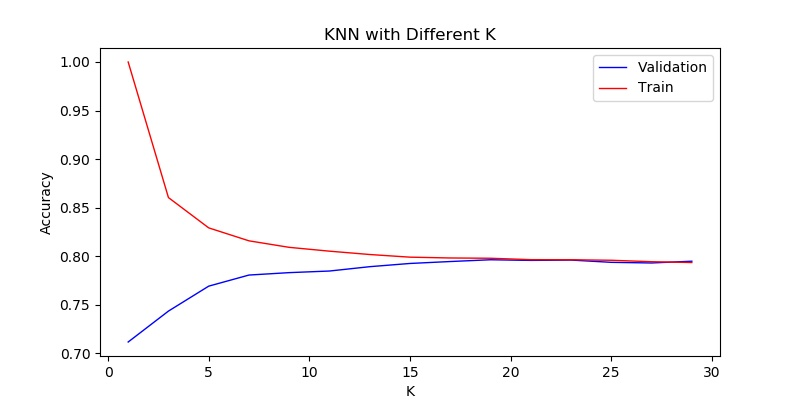
\includegraphics[width=\linewidth]{./adult/knn_k.jpg}
  \caption{Accuracy with Different K}
  \label{fig:adult_knn}
\end{figure}
We may conclude that when k is small, overfitting may happen since there is a large gap between training accuracy and validation accuracy. This is reasonable because if we only look at a small number of neighbors, there would be a higher error probability.\\
\\
For the selection of hyperparameter k, we may conclude that k=19 is good and the model achieves 79.63\% accuracy in testing dataset.

\subsection{Decision Tree}
For decision tree algorithm, the hyperparameters include max number of leaves, max depth, etc. Here I test on different choose of max number of leaves and I use information gain for the criterion. From Fig.\ref{fig:adult_dt}, we can see clearly that the accuracy raise up rapidly first when leaf number is very small. Then the accuracy raise up slowly. After the number of leaves is greater than 20, the accuracy almost does not change. This makes sense because when a decision tree can be fully produced, there is no use to increase the maximal number of leaves.
\begin{figure}[h!]
  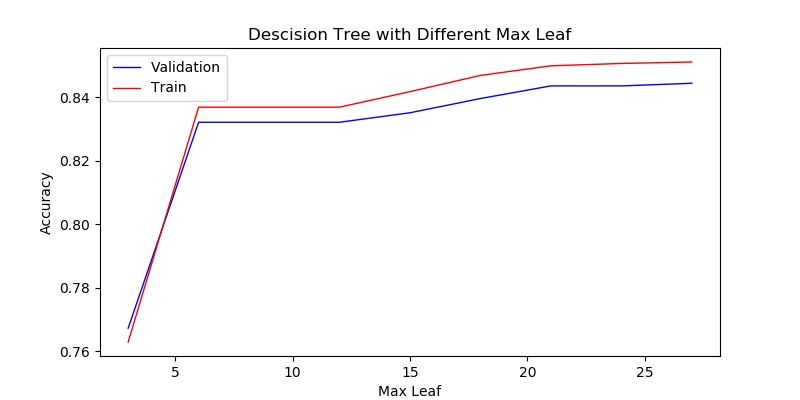
\includegraphics[width=\linewidth]{./adult/dt_maxleaf.jpg}
  \caption{Accuracy with Different Number of Max Leaves}
  \label{fig:adult_dt}
\end{figure}
We may conclude that when the maximal number of leaves is so small, increasing the maximal number can make the performance of the algorithm much better while when k becomes larger, the increase of the accuracy is not that obvious. I believe there is a trade-off between the complexity of the decision tree and the accuracy. If one want his decision tree to reach as higher accuracy as possible, he may choose to have no limitation on maximal number of leaves. On the contrary, if one would like to limit the complexity of his decision tree, he may just choose a reasonably small number as the limit. \\
\\
For the selection of this parameter, I choose max number equals 21 and the test accuracy is 84.40\%. The testing accuracy is actually very close to training and validation accuracy, which indicates that overfitting does not happen here.

\subsection{Boosting}
Ada boosting is used as boosting algorithm here. The hyperparameter I choose here is the number of estimators. From Fig.\ref{fig:adult_ada}, we can see that the training accuracy and validation accuracy both increase as the number of estimators increase. However, if we look at the data, the accuracy only increase in a small number. 
\begin{figure}[h!]
  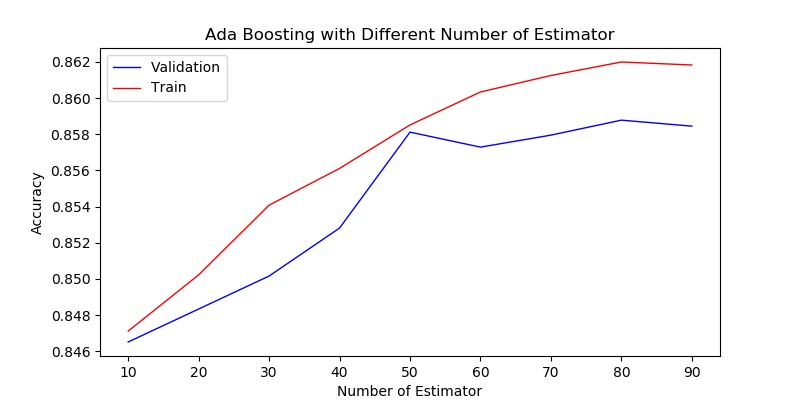
\includegraphics[width=\linewidth]{./adult/ada_num_estimator.jpg}
  \caption{Accuracy with Different Number of Estimators}
  \label{fig:adult_ada}
\end{figure}
We may conclude that the number of estimator does not have great influence on the algorithm but it is a good way to increase the accuracy after it reaches a high value.

\subsection{Support Vector Machine}
For support vector machine, I use four different kernel functions: poly, linear, rbf and sigmoid. The performace of each kernel function is shown in Fig.\ref{fig:adult_svm}. It is clear that rbf function is the best one among those four and sigmoid is the worst one. An interesting thing is that the gap between training accuracy and validation accuracy is very samll for all of these four algorithms.
\begin{figure}[h!]
  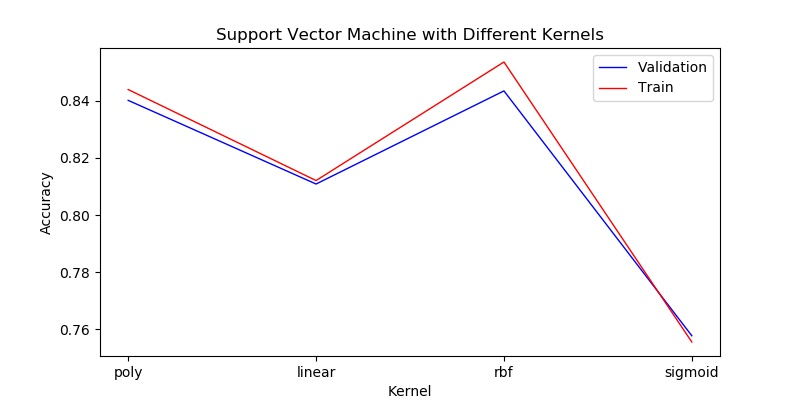
\includegraphics[width=\linewidth]{./adult/svm_kernel.jpg}
  \caption{Accuracy Using Different Kernel Function}
  \label{fig:adult_svm}
\end{figure}
I would say that support vector machine is a good algorithm because it seems overfiting may not happen.\\
\\
Using rbf as kernel function and the test accuracy is 83.22\%.

\subsection{Neural Network}
Neural network has many hyperparameters. I test on the number of hidden layers and fix other hyperparameters. From Fig\ref{fig:adult_nn}, it is clear that the accuracy of neural network is not stable. It first decreases as number of layers goes up and then increases. The best accuracy is attained when there are 19 hidden layers of neural network. 
\begin{figure}[h!]
  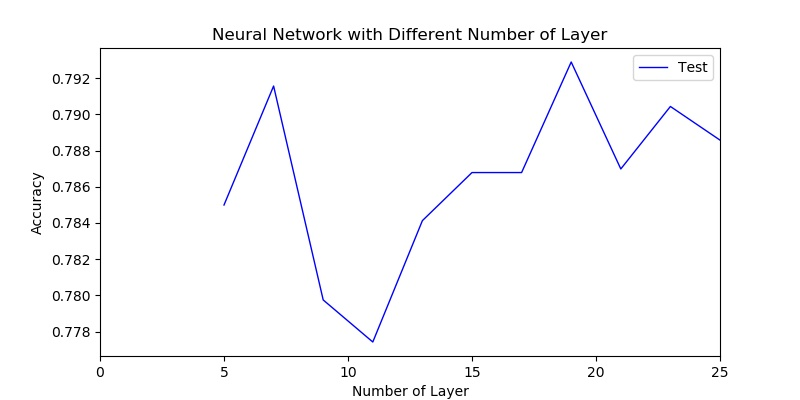
\includegraphics[width=\linewidth]{./adult/nn_num_layer.jpg}
  \caption{Accuracy with Different Number of Layers}
  \label{fig:adult_nn}
\end{figure}
It looks strange for me as the trend of accuracy with regard to the number of hidden layers is not consistent. Neural network seems to be a black box for me as I really don't know what happens inside the hidden neurons. \\
\\The only thing I can tell is that the test accuracy for neural network with 19 hidden layers is 78.86\%. It is not bad compared with other algorithms.

\subsection{Summary}
Table.\ref{tab:adult} shows the performance of different algorithms on test data. Decision tree seems to be the best algorithm for adult data and neural network does not work as well as other algorithms. At my first sight, it is contradictory to my experience that neural network is used broadly and has get excellent result. I think the point is that this dataset is a trivial one. The dimensions and size of the dataset is not complicated and traditional machine learning algorithms can handle this problem well.
\begin{table}[h!]
  \begin{center}
    \caption{Performance of Algorithms}
    \label{tab:adult}
    \begin{tabular}{l|c}
      \textbf{Algorithm} & \textbf{Testing Accuracy}\\
      \hline
      KNN & 79.47\%\\
      Decision Tree & 84.40\%\\
      Boosting & 82.34\%\\
      SVM & 83.23\% \\
      Neural Network & 78.86\%\\
    \end{tabular}
  \end{center}
\end{table}
As far as I know, neural network needs large scale data to get trained and the hyperparameters need to be set up correctly in order to have faster training speed and better accuracy. For this training set, neural network can get a good testing accuracy, but not the best. Other traditional machine learning algorithms work even better.\\
\\
For the running time of the algorithm, support vector machine takes the longest time, followed by neural network. Then comes k nearest neighbor and other two algorithms runs almost the same time. Boosting runs slightly faster. I do expect that neural network would take long time to train while I did not expect support vector machine to take that much time. The reason may be that the data is complicated and the computation for kernel function is expensive. The time of decision tree and boosting are close because boosting is just some accelaration of decision tree.
\section{Wine Dataset Classification and Result}
\subsection{K Nearest Neighbor}
Based on Fig.\ref{fig:wine_knn}, we can see that training score first decreases and then is somehow stable and the trend of validation score goes similarly. 
\begin{figure}[h!]
  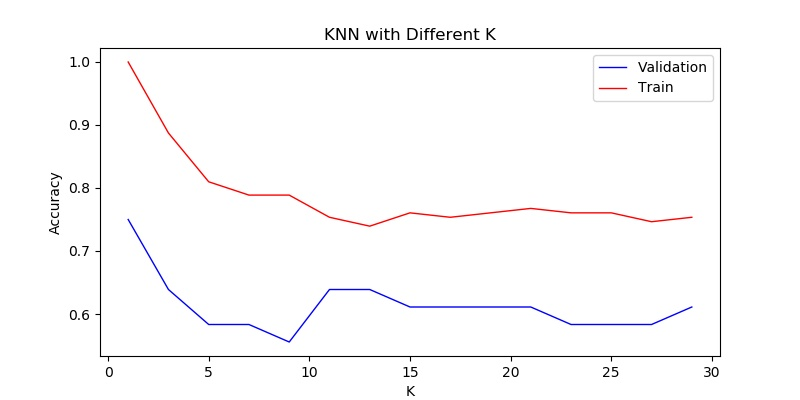
\includegraphics[width=\linewidth]{./wine/knn_k.jpg}
  \caption{Accuracy with Different k}
  \label{fig:wine_knn}
\end{figure}\\
The behavior of k nearest neighbor on wine dataset is different from that on adult dataset. For adult dataset, the validation score at the beginning is very low and increases afterwards. For my point of view, this is because wine dataset only contains a small number of data. I believe the overfitting happens while the validation set cannot show since the size of dataset is so small.
\subsection{Decision Tree}
Based on Fig.\ref{fig:wine_dt}, we can see the training accuracy reaches 100\% after max number of leaves is greater than 9! This indicates that the decision tree is fully built and the accuracy of validation set also supports it because the validation accuracy is extremely high and reaches around 97\%.
\begin{figure}[h!]
  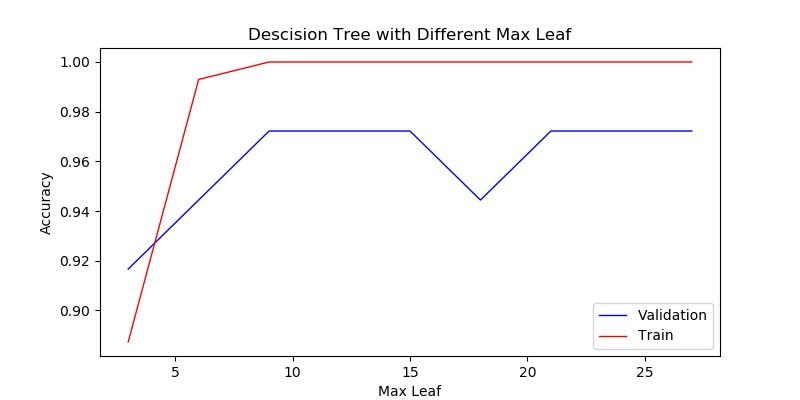
\includegraphics[width=\linewidth]{./wine/dt_maxleaf.jpg}
  \caption{Accuracy with Different Max Number of Leaves}
  \label{fig:wine_dt}
\end{figure}\\
The high accuracy indicates that decision tree algorithm may be extremely helpful when the problem space is not very large. The tree can even be fully obtained and the accuracy can be very high.

\subsection{Boosting}
It is strange for me that changing number of estimators does not change the training and validation accuracy. The line is shown on Fig.\ref{fig:wine_ada}. In my point of view, this supports my previous argue that the problem space is small and a decision tree can be fully obtained even without boosting. Also, the fact that the problem space is small supports the result of experiment. There would be no improvement between different number of estimators.
\begin{figure}[h!]
  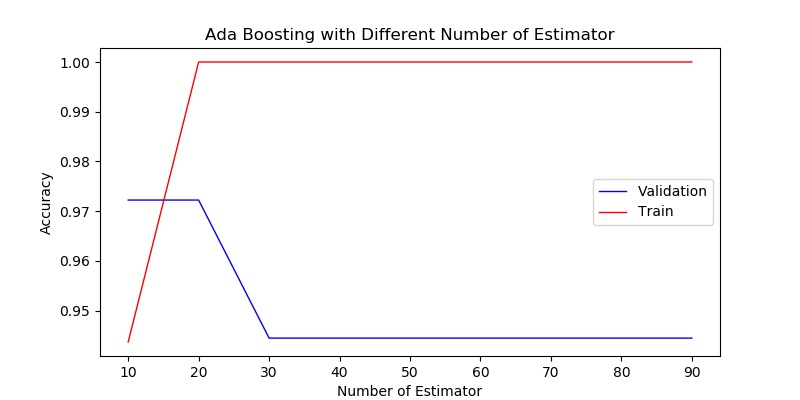
\includegraphics[width=\linewidth]{./wine/ada_num_estimator.jpg}
  \caption{Accuracy with Different Number of Estimators}
  \label{fig:wine_ada}
\end{figure}\\
\subsection{Support Vector Machine}
Again, support vector machine works well on wine dataset. Sigmoid kernel function even reach 100\% accuracy. Other kernel functions also have accuracy at around 97\%, which is as good as a fully obtained decision tree. Perhaps this is because different kinds of wines actually differs a lot in some properties and the support vector machine can successfully partition them easily. Imagine that the three types of wines are distributed among the space sparsely while the data points representing same kinds of wines are aggregated together. Then it is easy for a support vector machine to do classification.
\begin{figure}[h!]
  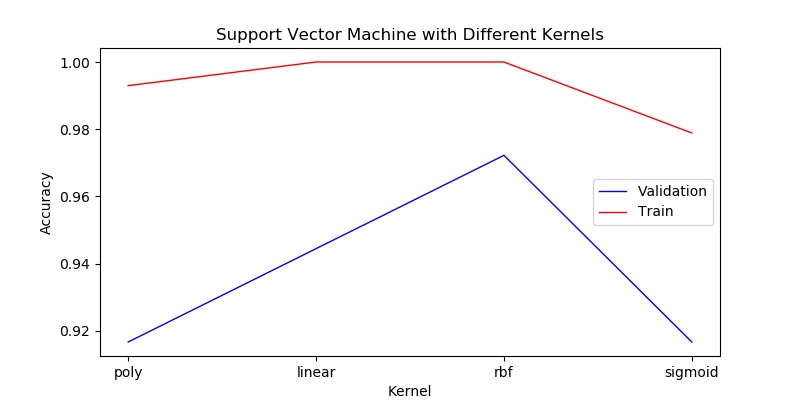
\includegraphics[width=\linewidth]{./wine/svm_kernel.jpg}
  \caption{Accuracy Using Different Kernel Function}
  \label{fig:wine_svm}
\end{figure}\\
\begin{figure}[h!]
  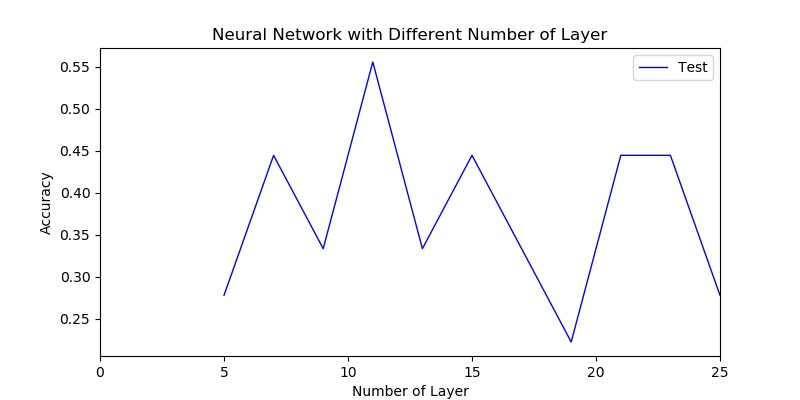
\includegraphics[width=\linewidth]{./wine/nn_num_layer.jpg}
  \caption{Accuracy with Different Number of Hidden Layers}
  \label{fig:wine_nn}
\end{figure}
\subsection{Neural Network}
Fig.\ref{fig:wine_nn} shows the accuracy with different number of hidden layers and each layer has 30 neurons. Unlike other algorithms, the performance of neural network is really bad on wine dataset. Considering the fact that random guess can reach 33.3\% accuracy, when hidden layers equals to some numbers, neural network behaves like a disaster. But this is actually what I expected. Since there are only 178 instances in total and I have to do cross validation, the size of training data may be only 130. The size of training data is so small for a neural network to be successfully trained. If we can find more training data and feed it to neural network, I believe that the accuracy can be much better than the current one. 
\subsection{Summary}
Table.\ref{tab:wine} shows the performance of different algorithms on test data. Decision tree and support vector machine seems to be the best algorithm for wine data and neural network does not work as well as other algorithms. Boosting and decision tree have the same accuracy because the tree can be fully obtained even without any boosting. From the accuracy of neural network, I can see that the performance of a machine learning algorithm is greatly related with the dataset. For adult data, the performance of neural network is acceptable while for wine data, neural network is much worse than traditional algorithms. The data size does influence the performance of different algorithms.\\
\begin{table}[h!]
  \begin{center}
    \caption{Performance of Algorithms}
    \label{tab:wine}
    \begin{tabular}{l|c}
      \textbf{Algorithm} & \textbf{Testing Accuracy}\\
      \hline
      KNN & 80.56\%\\
      Decision Tree & 97.22\%\\
      Boosting & 97.22\%\\
      SVM & 100.0\% \\
      Neural Network & 55.56\%\\
    \end{tabular}
  \end{center}
\end{table}\\
As for the running time, k nearest neighbor is now the slowest one, followed by neural network and support vector machine. Decision tree and boosting are the fastest. For my thought, k nearest neighbor takes some computation time for computing the nearest neighbors and then voting. Since the wine dataset does not contain much instances, neural network and support vector machine is fast this time. Decision tree and boosting are still the fastest because the main cost for these two algorithms is generating the tree, which can be easily done for wine dataset.

\section{Influence of Size}
For adult dataset, I will partition the dataset into training set and validation set with different factors and see how the size of training data influence the behavior of different algorithms. I do not do so for wine dataset since wine dataset only contains 178 instances and I believe it is meaningless to do so.
\begin{figure}[h!]
  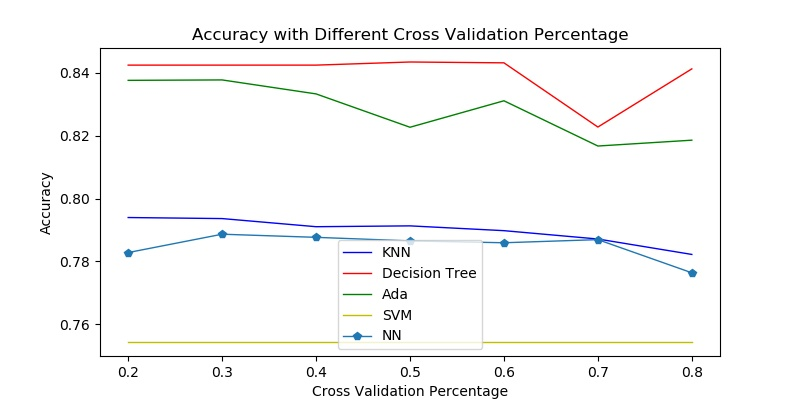
\includegraphics[width=\linewidth]{./adult/compare.jpg}
  \caption{Accuracy with Different Cross Validation Factor}
  \label{fig:compare}
\end{figure}\\
Fig.\ref{fig:compare} shows the change. We may conclude that decision tree and support vector machine is stable with decreasing size of training set while the accuracy of other algorithms are slightly influenced. It is clear that the accuracy for support vector machine even does not change. I believe it is because the data points are uniformly distributed. By "uniform" I mean that the data is spreaded among the space and decrease the size almost has no influence.

\end{document}
